%~~~~~~~~~~~~~~~~~~~~~~~~~~~~~~~~~~~~~~~~~~~~~~~~~~~~~~~~~~~~~~~~~~~~~~~
\section{Representação implícita probabilística de grafos}\label{sec:graphs}
%~~~~~~~~~~~~~~~~~~~~~~~~~~~~~~~~~~~~~~~~~~~~~~~~~~~~~~~~~~~~~~~~~~~~~~~

Estruturas de dados probabilísticas apresentam novas formas de aproximar a resposta de problemas clássicos sob um ponto de vista probabilístico. Apresentaremos, neste capítulo, ideias para representações probabilísticas de grafos utilizando estruturas descritas nos capítulos anteriores.

Spinrad mostra em \cite{spinrad2003efficient} que $\Theta(n^2)$ bits são necessários para representar qualquer grafo. Classes específicas de grafos, entretanto, podem possuir representações mais compactas. Discutimos sobre representações implícitas ótimas ao longo da Seção~\ref{sec:graphs:implicit}.

Os resultados em \cite{pell2012scaling} e \cite{zhang2014these} mostram o uso de estruturas probabilísticas (Filtros de Bloom, \emph{Count-Min Sketch} para a montagem de fragmentos de genoma bacterial. Discutimos estes resultados na Seção~\ref{sec:graphs:genome}

Por fim, discutimos na seção~\ref{sec:graphs:repres} novas ideias para representações probabilísticas de grafos que podem diminuir a complexidade de espaço para representar algumas classes de grafos.

\subsection{Introdução a representações implícitas}\label{sec:graphs:implicit}

Nesta seção, apresentamos conceitos sobre representações eficientes de grafos. Esta área baseia-se muito nos trabalhos de Muller \cite{muller1988local} e Kannan, Naor e Rudich \cite{kannan1992implicat}, entretanto, o livro de Spinrad \cite{spinrad2003efficient} sintetizou bem a teoria descrita até o momento, motivando novos trabalhos na área.

Para fins de notação, dizemos que um grafo $G$ é denotado pela tupla $(V, E)$, onde $V$ é o conjunto de vértices, de cardinalidade $n = |V|$ e $E$ é o conjunto de arestas, de cardinalidade $m = |E|$. Cada aresta é um par não-ordenado $(u, v) \mid u,v \in V$. A maior parte das discussões nesta seção aplicam-se a grafos rotulados (onde grafos isomórficos com rótulos diferentes são considerados grafos diferentes).

Começamos por discutir as duas representações clássicas de grafos: matriz de adjacência e lista de adjacência. 

A matriz de adjacência utiliza $\Theta(n^2)$ bits para representar a presença ou ausência de todas as possíveis arestas entre dois vértices no grafo. A vantagem desta representação é a possibilidade de testar a adjacência entre dois vértices em tempo constante.

A lista de adjacência mantém, para cada vértice $v$, uma lista dos vértices $u$ tal que $(u, v) \in E$. Para representar um grafo, $n$ listas são mantidas com um total de $2m$ itens (pois cada aresta aparece em exatamente duas listas). Cada item pode ser denotado por número no intervalo $[1..n]$, precisando, portanto de $O(\log n)$ bits para ser representado. Assim, a lista de adjacência representa um grafo de $n$ vértices utilizando $O(m \log n)$ bits.

Cada uma dessas representações tem vantagens e desvantagens. Por exemplo, não é possível testar a conectividade do grafo em tempo linear ($O(n + m)$) utilizando apenas uma matriz de adjacência. Com uma lista de adjacência seria possível fazê-lo, o que apresenta grande vantagem no caso de grafos esparsos, entretanto o teste de adjacência nesta representação requer tempo no mínimo logarítmico. É possível, no entanto, analisar qual das representações é ótima em espaço para representação de grafos em geral. Neste contexto, uma representação é ótima se requer $O(f(n))$ bits para representar uma classe contendo $2^{\Theta(f(n))}$ grafos de $n$ vértices.

Por exemplo, é possível provar que existem $2^{\Theta(n^2)}$ grafos com $n$ vértices, pois há $n (n-1)/2$ arestas possíveis e cada grafo é uma combinação destas. Existem portanto, $2^{n (n-1) / 2}$ grafos rotulados de $n$ vértices, isto é $2^{\Theta(n^2)}$. O mesmo argumento serve para grafos não-rotulados, pois para cada grafo existem no máximo $n!$ isomorfismos, isto é, existem pelo menos $2^{n (n-1) / 2} / n!$ grafos não-isomorfos. Como $n!$ é $2^{\Theta(n \log n)}$, então segue que o número e grafos não-isomorfos é $2^{\Theta(n^2)}$.

Desta forma, diz-se que a matriz de adjacência representa otimamente a classe contendo todos os grafos (rotulados ou não), pois requer $O(n^2)$ bits para representar uma classe contendo $2^{\Theta({n^2})}$ grafos. Já a lista de adjacência não é ótima, pois no caso de grafos completos, requer $\Theta(n^2 \log n)$ bits.

Muitas vezes, a representação escolhida altera a complexidade de certos problemas sobre o grafo que elas representam. Em \cite{dahlhaus2002partially}, Dahlhaus at al. introduzem uma representação derivada de uma lista de adjacência onde a lista relativa a cada vértice possui um bit que define se a lista representa as adjacências do vértice no grafo original ou em seu complemento. O trabalho mostra também que é possível computar diversos algoritmos sobre o complemento do grafo com tempo linear sobre a representação, já que a representação de um grafo $G$ e seu complemento $\overline{G}$ são iguais.

Para classes de grafos com $2^{O(n\log n)}$ elementos, uma representação ótima deve ter $O(n\log n)$ bits. Entretanto, apenas esta propriedade não é suficiente para garantir sua eficiência. Por exemplo, uma representação genérica ótima poderia ser definida enumerando todos os grafos em uma certa classe C, que possui $2^{\Theta(f(n))}$ elementos, e usar este número de $\Theta(f(n))$ bits como representação. Entretanto, esta representação não permitiria que teste de adjacência fosse realizado sem recriar o grafo original. De fato, seria necessário reconstruir o grafo a partir da representação para testar a adjacência entre vértices.

Em um exemplo prático, é trivial mostrar que existem $2^{O(n\log n)}$ árvores, pois sua representação como lista de adjacência usa $O(n \log n)$ bits. Esta representação, entretanto, não favorece o teste de adjacência, pois a lista de cada vértice pode ter $O(n \log n)$ bits. Uma representação mais apropriada seria definir um vértice arbitrário como raiz da árvore e manter, para cada vértice, apenas seu pai nesta arborescência. Assim, apenas $O(\log n)$ bits são necessários para cada vértice e o teste de adjacência entre vértices pode ser feito de forma eficiente, apenas verificando se um dos vértices é pai do outro na representação. Um exemplo desta representação pode ser visto na Figura~\ref{fig:graphs1}. 

\begin{figure}[!htbp]
  \centering
  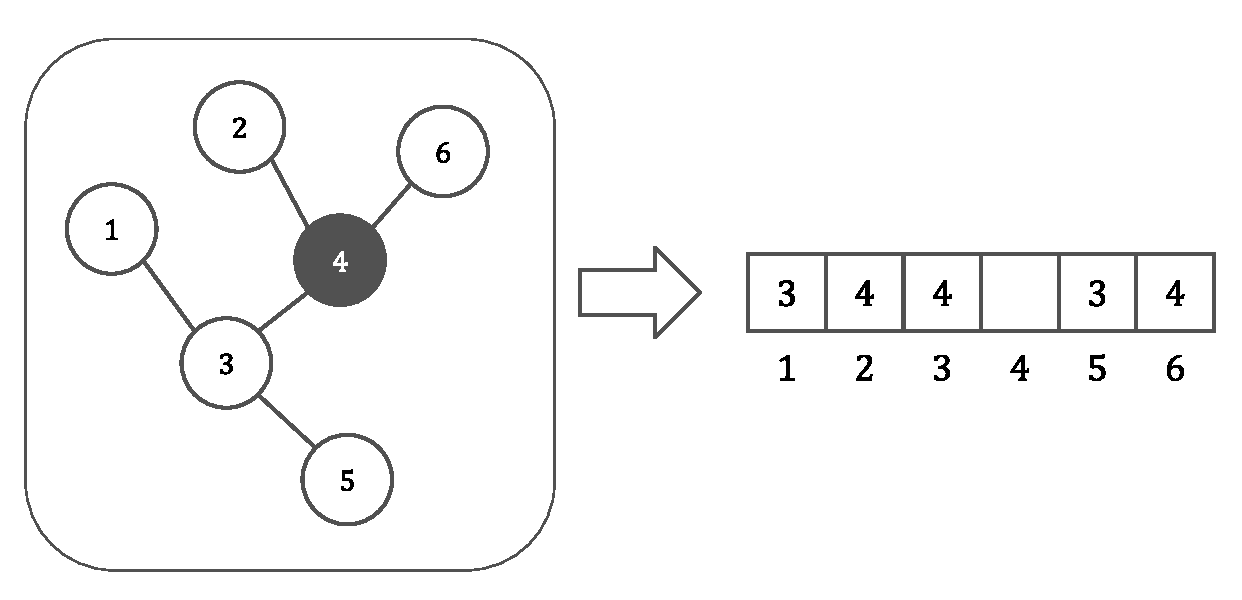
\includegraphics[scale=0.6]{files/graphs1.pdf}
  \caption{Exemplo de representação implícita de árvores, com vértice raiz realçado}
  \label{fig:graphs1}
\end{figure}

Esta \emph{eficiência} do teste de adjacência parece estar ligada ao fato da representação manter um número limitado de bits para cada vértice e utilizar apenas estes bits para o teste. Assim, podemos definir intuitivamente o conceito de representação implícita \footnote{Na literatura é usual definir como representação implícita apenas aquelas com $f(n) = n \log n$. A definição que apresentamos aqui é uma versão generalizada, formalizada em \cite{spinrad2003efficient}, que é mais apropriada para os problemas que trataremos a frente.} como a seguir:

Seja $C$ uma classe de grafos com $2^{\Theta(f(n))}$ elementos. Uma representação $R$ de um grafo $G \in C$, de $n$ vértices é dita implícita se:
\begin{enumerate}  
\item \emph{ela é assintoticamente ótima:} a representação requer apenas $O(f(n))$ bits no total;
\item \emph{ela distribui informação entre os vértices:} a representação local de cada vértice possui apenas $O(f(n)/n)$ bits;
\item \emph{o teste de adjacência é local:} para testar a adjacência entre dois vértices, apenas as informações locais a eles são necessárias.
\end{enumerate}

Um exemplo de classe que respeita essas propriedades são os \emph{grafos de intervalo}. Um grafo é dito de intervalo se cada um de seus vértices puder ser mapeado para um intervalo na reta real. Há aresta entre dois vértices se e somente se os respectivos intervalos possuem uma interseção não-vazia. Esta classe possui grande utilidade prática e pode ser definida uma representação implícita simples baseada na definição da classe. 

A representação consiste em enumerar as extremidades dos intervalos, na ordem em que aparecem na reta real, com inteiros no intervalo $[1..2n]$. Representa-se cada vértice do grafo com os dois inteiros correspondentes às extremidades de seu respectivo intervalo. Um exemplo pode ser visto na Figura~\ref{fig:graphs2}. Dois vértices serão considerados adjacentes se e somente se os intervalos representados pelos inteiros possuírem interseção não-vazia. Apenas $\Theta(\log n)$ bits são usados para representar cada vértice e $\Theta(n\log n)$ bits são usados para representar o grafo inteiro. Isto indica que há $2^{O(n \log n)}$ grafos de intervalo possíveis.

\begin{figure}[!htbp]
  \centering
  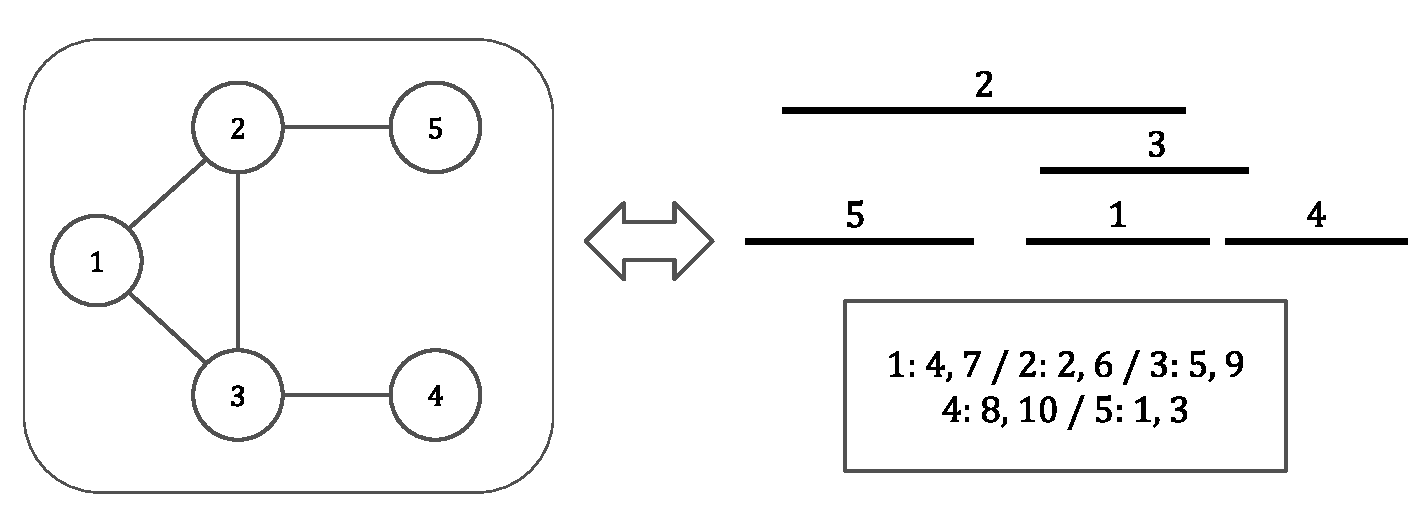
\includegraphics[scale=0.6]{files/graphs2.pdf}
  \caption{Exemplo de representação implícita de grafos de intervalo}
  \label{fig:graphs2}
\end{figure}


Para verificar o limite inferior no número de elementos na classe, considere grafos com $n$ vértices onde cada um dos $n/2$ primeiros vértices possuem uma aresta para um vértice distinto entre os $n/2$ últimos. Esta é uma subclasse dos grafos de intervalo. Por definição, ela possui $(n/2)!$ possíveis grafos com $n$ vértices. Como, $(n/2)!$ é $2^{\Theta(n \log n)}$, segue que há $2^{\Theta(n \log n)}$ grafos de intervalo e, portanto, a representação apresentada anteriormente é ótima.

Encontrar uma representação que respeite as propriedades necessárias pode não ser trivial. De fato, para muitas classes pode ser que não exista representação implícita. Por exemplo, considere a classe de grafos onde $m \leq n$. Usando uma lista de adjacência, é possível representar grafos nesta classe usando $O(n \log n)$ bits, o que indica que esta classe possui $2^{O(n\log n)}$ elementos. É impossível, entretanto, satisfazer as propriedades (2) e (3) simultaneamente, pois é possível transformar um grafo qualquer para um nesta classe introduzindo $n^2$ vértices de grau zero. Assim, se fosse houvesse uma representação implícita para este grafo, seria possível representar os $n$ vértices originais e suas adjacências usando apenas $O(n \log n)$ bits. Isto implicaria que é possível representar qualquer grafo usando $O(n \log n)$ bits, o que é absurdo.

A possibilidade de construir grafos em classes com $2^{\Theta(n\log n)}$ grafos a partir de grafos gerais apenas adicionando vértices pode posar como um desafio para definir propriedades gerais sobre essas classes. Por isso, utiliza-se mais frequentemente classes hereditárias na busca por classes com representações implícitas.

Uma classe é dita \emph{hereditária} se para todo grafo $G$ nesta classe, todo subgrafo induzido de $G$ também está na classe. A classe definida anteriormente (onde $m \leq n$) não é hereditária, pois a remoção de vértices de grafos naquela classe pode resultar em grafos fora dela. É possível provar que uma classe hereditária $C$ contém $2^{\Theta(n^2)}$ se e somente se ela contém todos os grafos bipartidos, todos os co-bipartidos ou todos os grafos \emph{split}.

É uma conjectura aberta se toda classe hereditária com $2^{O(n \log n)}$ grafos possui uma representação implícita. É conhecida como \emph{Conjectura da Representação Implícita} \cite{kannan1992implicat,spinrad2003efficient,chandoo2016implicit}. Importante notar que mesmo classes não-hereditárias podem possuir representação implícita (por exemplo, árvores).

%INCLUIR ALGO SOBRE REPRESENTAÇÕES PROBABILÍSTICAS

\subsection{Filtro de Bloom como representação implícita}\label{sec:graphs:repres}

Os resultados em \cite{pell2012scaling} e \cite{zhang2014these} suscitam a discussão sobre a viabilidade de representações probabilísticas para outras classes de grafos além dos de Bruijn.

Nesta seção, exploramos representações alternativas de grafos que utilizam estruturas de dados probabilísticas para permitir a estimativa das relações de adjacência entre os vértices. Deseja-se que, para determinadas classes de grafos, estas representações sejam pelo menos tão eficientes quanto as melhores representações conhecidas. Isto é, se uma classe $C$ possui $2^{\Theta(f(n))}$ grafos, o objetivo é derivar representações probabilísticas que requeiram $O(f(n))$ bits e permitam teste de adjacência com erro relativo constante $\epsilon$ e confiança $1 - \delta$.

Como exemplo, podemos estudar o uso direto de filtros de Bloom para representação do conjunto de arestas $E$ em grafos gerais. Como o objetivo é representar grafos gerais, o desejável é que seja possível construir o filtro com complexidade igual ou (preferencialmente) inferior a $\Theta(n^2)$. 

A ideia consiste em encontrar uma função \emph{hash} $h: E \to [1..m_B]$, que mapeia arestas do grafo em posições em um filtro de Bloom de $m_B$ bits.

De fato, filtros de Bloom permitem representar toda a adjacência do grafo utilizando 10 bits por aresta -- isto é, O(m) bits --, a fim de alcançar uma probabilidade de falsos positivos menor que 1\%. Esta representação mostra grande valor para representação de grafos esparsos, apesar de ser igualmente eficiente à matriz de adjacência ao requerer $\Theta(n^2)$ bits para representar o grafo no pior caso (ex.: grafos completos).

Esta representação possui uma característica importante: toda aresta do grafo é representada deterministicamente. Isto é, se a aresta existe no grafo original, com 100\% de probabilidade ela existirá na versão probabilística. Desta propriedade, segue que se um teste de adjacência na representação probabilística resultar em resposta negativa, é garantido que a aresta não exista no grafo original. Isto é, como característica do filtro de Bloom, não há falsos negativos. O contrário, entretanto, não é verdade. Em testes de adjacência entre vértices não-adjacentes, há probabilidade de falsos positivos. Isto significa, que para uma probabilidade de falsos positivos $p$, espera-se encontrar $p(\frac{n(n-1)}{2}-m)$ arestas na representação probabilística que não existem no grafo original.

É importante notar que, construída da forma apresentada, esta não seria uma representação implícita, mesmo se relaxarmos o requisito do teste de adjacência para permitir respostas probabilísticas. Isto se deve a esta representação não distribuir a informação entre os vértices. De fato, não há representação local nos vértices.

Uma variação que resolveria este problema seria manter um filtro de Bloom para cada vértice. Assim, para cada vértice $v$, teríamos um filtro de Bloom com $10 \times \text{d}(v)$ bits -- onde $\text{d}(v)$ é o grau do vértice -- de forma que a probabilidade de falsos positivos em cada um deles é exatamente igual e equivalente à versão anteriormente apresentada. Assim, para cada vértice, esta representação necessita de $O(\text{d}(v))$ bits que, no pior caso, é equivalente à matriz de adjacência ($O(n)$ bits), entretanto, permite representação de grafos esparsos com complexidade menor que a lista de adjacência, que requer $O(\text{d}(v) \log n)$ bits.

A Figura~\ref{fig:graph:bloom} compara os resultados empíricos para sucessivos testes em grafos aleatórios com $n = 1000$ e $m$ variando em todos os valores possíveis para um grafo com este tamanho. Ambas as variantes apresentadas nesta seção foram testadas. Note que para $m=0$, por característica da construção filtro de Bloom, não há arestas espúrias.

\begin{figure}[!htbp]
\centering
\scalebox{0.80}{\begin{tikzpicture}[
        declare function = {
            p(\n,\m) = 0.008193722*(\n*(\n-1)/2-\m);
        }
    ]
	\begin{axis}[
	    title=Filtro de Bloom único,
	    scaled ticks=false, 
        grid=both,
        ylabel={arestas espúrias},
    	xlabel=número de arestas ($m$),
        xmin=0, xmax=5000,
        ymin=0, ymax=50,
		legend columns=1, 
	    legend style={legend pos=outer north east,}
    ]

	\addplot[line width=1pt, mark=*,black,smooth, mark options={scale=0.75}] table[x=m,y=v1] {files/graph_bloom.txt};
	\addplot[smooth, mark options={scale=0.75}, line width=5pt,color={rgb:black,1;white,1},opacity=0.4] table[x=m,y=e] {files/graph_bloom.txt};
    %\addplot[dotted, line width=1pt, mark=none,black,smooth] table[x=k,y=max] {files/minhash_shakespeare.txt};
	%\legend{esperado,shakespeare, $\pm 1 \sigma$, min/max };


	\end{axis}
\end{tikzpicture} \begin{tikzpicture}[
        declare function = {
            p(\n,\m) = 0.008193*(\n*(\n-1)/2-\m);
        }
    ]
	\begin{axis}[
	    title=Um fitro de Bloom para cada vértice,
	    scaled ticks=false, 
        grid=both,
        xmin=0, xmax=5000,
        ymin=0, ymax=50,
		xlabel=número de arestas ($m$),
		yticklabel={\ },
		legend columns=1, 
	    %legend style={legend pos=outer north east,}
    ]

	\addplot[line width=1pt, mark=*,black,smooth, mark options={scale=0.75}] table[x=m,y=v2] {files/graph_bloom.txt};
	\addplot[smooth, mark options={scale=0.75}, line width=5pt,color={rgb:black,1;white,1},opacity=0.4] table[x=m,y=e] {files/graph_bloom.txt};
    %\addplot[dotted, line width=1pt, mark=none,black,smooth] table[x=k,y=max] {files/minhash_shakespeare2.txt};
	\legend{observado, esperado};

	\end{axis}
\end{tikzpicture}}
\caption{Arestas espúras em um grafo com $n=1000$.}
\label{fig:graph:bloom}
\end{figure}

\subsection{\emph{MinHash} como representação implícita}

